Empleando el montaje experimental descrito, se obtuvieron las curvas
características de fotocorriente \(I_p\) en función del potencial \(V\)
para la fotocelda, presentadas en las \cref{fig:blue-data,fig:violet-data}.
En el caso del filtro azul, los datos corresponden a tres intensidades
lumínicas distintas, mientras que para el filtro violeta solo se
registraron dos. Esto se debe a que, para la intensidad \(I_2\), el
cambio de polaridad falló durante la adquisición de datos, impidiendo
la determinación del potencial de frenado en dicho caso.

\begin{figure}[htbp!]
\begin{center}
  \includegraphics[width=0.9\linewidth, page=2]{../Images/characteristics.pdf}
  \caption{Curva característica de la fotocelda con filtro azul.}
  \label{fig:blue-data}
\end{center}
\end{figure}

\begin{figure}[htbp!]
\begin{center}
  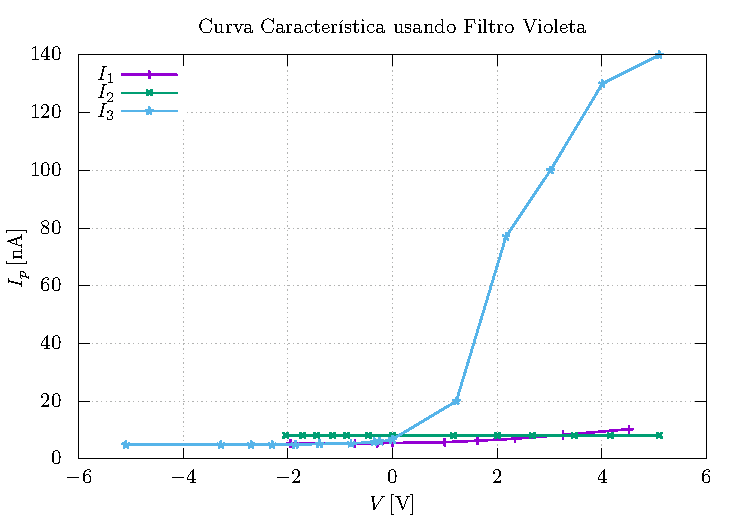
\includegraphics[width=0.9\linewidth, page=1]{../Images/characteristics.pdf}
  \caption{Curva característica de la fotocelda con filtro violeta.}
  \label{fig:violet-data}
\end{center}
\end{figure}

Las gráficas muestran que la intensidad lumínica \(I\) es proporcional
a la magnitud de la fotocorriente \(I_p\), en concordancia con la teoría,
pues una mayor intensidad implica un mayor número de fotones capaces de
generar el efecto. Sin embargo, la intensidad lumínica no influye en el
valor del potencial de frenado, como se observa en ambos filtros.

Otro aspecto a considerar es que, en igualdad de condiciones, se esperaría
una mayor magnitud de \(I_p\) con el filtro violeta que con el azul.
No obstante, debido a las condiciones experimentales, no es posible comparar
directamente dichas magnitudes, ya que las intensidades lumínicas no fueron
equivalentes.

Debido al desconocimiento de las especificaciones exactas de los filtros
utilizados, se estimaron la longitud de onda \(\lambda\) y la frecuencia \(\nu\)
de la luz incidente a partir del color del filtro bajo iluminación blanca y su
comparación con valores reportados en la literatura \cite{bruno2005crc}.
Los valores de \(\lambda\), \(\nu\) y el potencial de frenado \(V_0\)
para cada filtro se presentan en la \cref{tab:V0-data}.

\begin{table}[htbp!]
  \centering
  \rowcolors{2}{white}{gray!25}
  \begin{tabular}{c|S[table-format=3.0]|S[table-format=3.0]|S[table-format=1.2(2)]}
    \toprule
    Filtro & {\(\lambda \, [\si{\nano\metre}]\)} & {\(\nu \, [\si{\tera\Hz}]\)} & {\(V_0 \, [\si{\volt}]\)} \\
    \midrule
    Azul & 500 & 600 & 0.84(1) \\
    Violta & 405 & 740 & 1.40(1) \\
    \bottomrule
  \end{tabular}
  \vspace{1.5pt}
  \caption{Potencial de frenado según el filtro utilizado.}
  \label{tab:V0-data}
\end{table}

Se observa que, a mayor frecuencia de la luz incidente, mayor es la magnitud
del potencial de frenado, en concordancia con el postulado de Planck, \cref{eq:planck-postulate},
según el cual la energía de un fotón es proporcional a su frecuencia.

Por último, se grafica el potencial de frenado en función de la frecuencia.
De acuerdo con la \cref{eq:K-energy}, la curva que une los puntos es una
línea recta cuya pendiente corresponde a la constante de Planck \(h\), y
su intercepto con el eje \(y\) representa la función trabajo de la fotocelda.

Los datos experimentales y el ajuste lineal se presentan en la \cref{fig:h-constant}.
Dado que solo se cuentan con dos puntos y dos parámetros a ajustar (pendiente e
intercepto), el error computacional del ajuste es nulo.

\begin{figure}[htbp!]
\begin{center}
  \includegraphics[width=0.9\linewidth, page=3]{../Images/characteristics.pdf}
  \caption{Energía cinética de los electrones en función de la frecuencia.}
  \label{fig:h-constant}
\end{center}
\end{figure}

El ajuste lineal proporciona un valor de \( h = \qty{4.00}{\eV\s} \), con un error
relativo porcentual del \qty{3}{\percent} respecto al valor de referencia
\qty{4.136}{\eV\s} reportado en la literatura \cite{bureau-international-des-poids-et-mesures-2018}.
Por otro lado, la función de trabajo obtenida es \(\phi = \qty{1.56}{\eV}\).

A partir de las \cref{eq:ν0-umbral,eq:λ0-umbral}, se determina una
frecuencia umbral de \(\nu_0 = \qty{390}{\tera\Hz}\) y una longitud de onda
umbral de \(\lambda_0 = \qty{766}{\nano\metre}\), correspondiente a una onda
electromagnética en el infrarrojo \cite{bruno2005crc}.

Estos valores son inesperados y se alejan de los resultados conocidos, ya que el
metal con la menor función de trabajo reportada para el efecto fotoeléctrico es
el cesio (\ce{Cs}), con \qty{1.9}{\eV} \cite{holzl-1979}.
